\documentclass[tikz,border=5pt]{standalone}
\usepackage{amsmath}
\usepackage{xcolor}
\usetikzlibrary{arrows.meta,backgrounds,calc,fit,positioning}
\definecolor{ink}{HTML}{0F172A}
\definecolor{mutedInk}{HTML}{475569}
\definecolor{lineGray}{HTML}{CBD5E1}
\definecolor{panelGray}{HTML}{F8FAFC}
\definecolor{summaryGray}{HTML}{F1F5F9}
\definecolor{operationTeal}{HTML}{0F766E}
\definecolor{operationFill}{HTML}{ECFEFF}
\definecolor{schemaViolet}{HTML}{6D28D9}
\definecolor{schemaFill}{HTML}{F5F3FF}
\definecolor{resultGreen}{HTML}{15803D}
\definecolor{resultFill}{HTML}{F0FDF4}

\tikzset{
  state card/.style={
    draw=mutedInk,
    fill=white,
    rounded corners=1.5mm,
    line width=0.55pt,
    font=\sffamily\small,
    align=center,
    inner sep=3mm,
    text=ink
  },
  concept card/.style={
    state card,
    fill=panelGray
  },
  summary card/.style={
    state card,
    fill=summaryGray
  },
  operation card/.style={
    draw=operationTeal,
    fill=operationFill,
    rounded corners=4mm,
    line width=0.75pt,
    font=\sffamily\small\bfseries,
    align=center,
    inner xsep=4mm,
    inner ysep=2.2mm,
    text=operationTeal
  },
  schema ref/.style={
    draw=schemaViolet,
    fill=schemaFill,
    double=schemaViolet,
    double distance=1pt,
    rounded corners=1mm,
    line width=0.65pt,
    font=\sffamily\bfseries,
    inner xsep=5mm,
    inner ysep=2.5mm,
    text=schemaViolet
  },
  result card/.style={
    state card,
    draw=resultGreen,
    fill=resultFill,
    text=resultGreen,
    line width=0.75pt
  },
  bank card/.style={
    draw=schemaViolet,
    fill=white,
    rounded corners=2mm,
    line width=0.75pt,
    inner sep=4mm,
    text=ink
  },
  meta edge/.style={
    -{Stealth[length=2mm]},
    densely dashed,
    draw=mutedInk,
    line width=0.6pt
  },
  process edge/.style={
    -{Stealth[length=2.2mm]},
    draw=ink,
    line width=0.85pt
  },
  section label/.style={
    font=\sffamily\scriptsize\bfseries,
    text=mutedInk,
    align=left
  }
}


\begin{document}
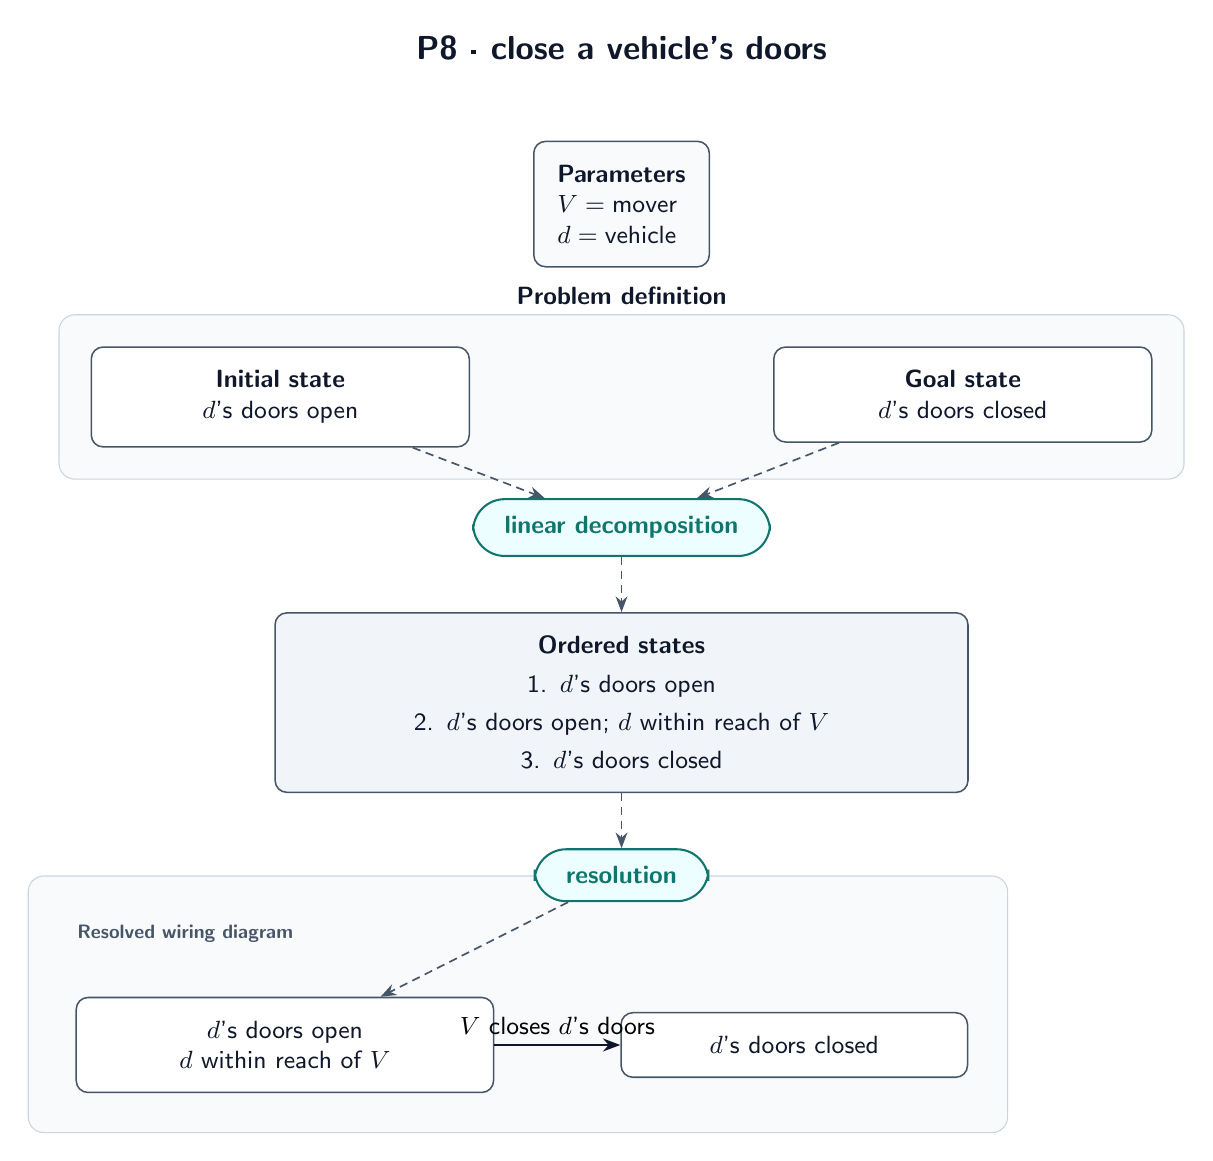
\begin{tikzpicture}[node distance=7mm]
  \node[concept card,align=left] (params) {
    \textbf{Parameters}\\
    $V=\text{mover}$\\
    $d=\text{vehicle}$
  };

  \node[state card,text width=42mm,below left=10mm and 8mm of params] (initial) {
    \textbf{Initial state}\\
    $d$'s doors open
  };
  \node[state card,text width=42mm,below right=10mm and 8mm of params] (goal) {
    \textbf{Goal state}\\
    $d$'s doors closed
  };
  \begin{scope}[on background layer]
    \node[draw=lineGray,fill=panelGray,rounded corners=2mm,
          fit=(initial)(goal),inner sep=4mm,
          label={[font=\sffamily\small\bfseries,text=ink]above:Problem definition}] {};
  \end{scope}

  \coordinate (problem-center) at ($(initial)!0.5!(goal)$);
  \node[operation card,below=13mm of problem-center] (decompose) {linear decomposition};
  \node[summary card,text width=82mm,below=of decompose] (states) {
    \textbf{Ordered states}\\[1mm]
    1. $d$'s doors open\\[1mm]
    2. $d$'s doors open; $d$ within reach of $V$\\[1mm]
    3. $d$'s doors closed
  };
  \node[operation card,below=of states] (resolve) {resolution};

  \node[state card,text width=47mm,below left=12mm and 5mm of resolve] (ready) {
    $d$'s doors open\\
    $d$ within reach of $V$
  };
  \node[state card,text width=38mm,right=16mm of ready] (closed) {
    $d$'s doors closed
  };
  \node[section label,anchor=west] (wiring-heading)
    at ($(ready.north west)+(-1mm,8mm)$) {Resolved wiring diagram};
  \begin{scope}[on background layer]
    \node[draw=lineGray,fill=panelGray,rounded corners=2mm,
          fit=(wiring-heading)(ready)(closed),inner sep=5mm] {};
  \end{scope}

  \draw[meta edge] (initial) -- (decompose);
  \draw[meta edge] (goal) -- (decompose);
  \draw[meta edge] (decompose) -- (states);
  \draw[meta edge] (states) -- (resolve);
  \draw[meta edge] (resolve) -- (ready);
  \draw[process edge] (ready) -- node[above,font=\sffamily\small] {$V$ closes $d$'s doors} (closed);

  \node[font=\sffamily\large\bfseries,text=ink,above=9mm of params] {
    P8 · close a vehicle's doors
  };
\end{tikzpicture}
\end{document}
